\documentclass[plain,basic]{inVerba-notes}

\newcommand{\userName}{Cullyn Newman}
\newcommand{\class}{BI:\@ 428}
\newcommand{\theTitle}{Journal Article Summary --- Week 2}
\newcommand{\institution}{Portland State University}

\begin{document}
\large{\textbf{Chromosome Conformation Capture and Beyond: Toward an Integrative View of Chromosome Structure and Function}}

\small{Authors: Rachel Patton McCord, Noam Kaplan, and Luca Giorgetti\\
\href{https://doi.org/10.1016/j.molcel.2019.12.021}{\bbb{https://doi.org/10.1016/j.molcel.2019.12.021}}}

\vspace{-12pt}
\subsubsection{Key Points}
\begin{itemize}
    \item New alternative techniques have emerged to study genome architecture and biological processes in the nucleus, often in single or living cells; allowing for exploring links between chromosome structure and biological function.
    \item Emphasis on understanding the 3D structure of chromosomes is important due to intimate interactions in 3D space with other mechanisms and how changes in shape affect such interactions.
    \item This study reviews popular as well as emerging approaches then discusses the next tech frontiers.
\end{itemize}

\vspace{-20pt}

\subsubsection{Introduction}
\begin{itemize}
    \item Current knowledge of 3D chromosomes structure derives from two complementary classes or techniques:
    \begin{itemize}
        \item Microscopy, which revealed many principles or nuclear organization including the existence of sub-nuclear organelles.
            \begin{itemize}
                \item Electron microscopy has extended understanding of fine-scale structure, but remains incompatible with sequence determination.
            \end{itemize}
        \begin{center}
            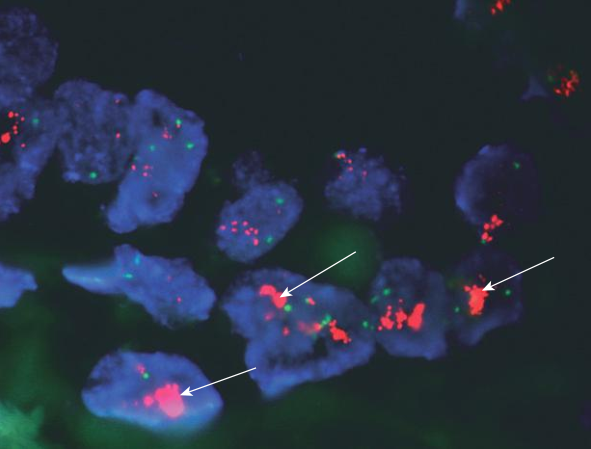
\includegraphics[scale=0.3]{images/fish.png}
        \end{center}
        \item Fluorescence RNA and DNA \textit{in situ} hybridization (FISH), which revealed that chromosomes occupy distinct chromosome territories and that nuclear positioning can correlate with gene expression levels.
            \begin{itemize}
                \item Live cell fluorescence microscopy lead to insights into the dynamic properties of chromosome organization and has begun to reveal how it relates to transcription through the direct visualization of the position and arrangement of chromosomes in the nucleus. 
                \item Limited in throughput as well as genomic and spatial resolution.
            \end{itemize}
    \end{itemize}
    \vspace{20pt}

    \begin{center}
        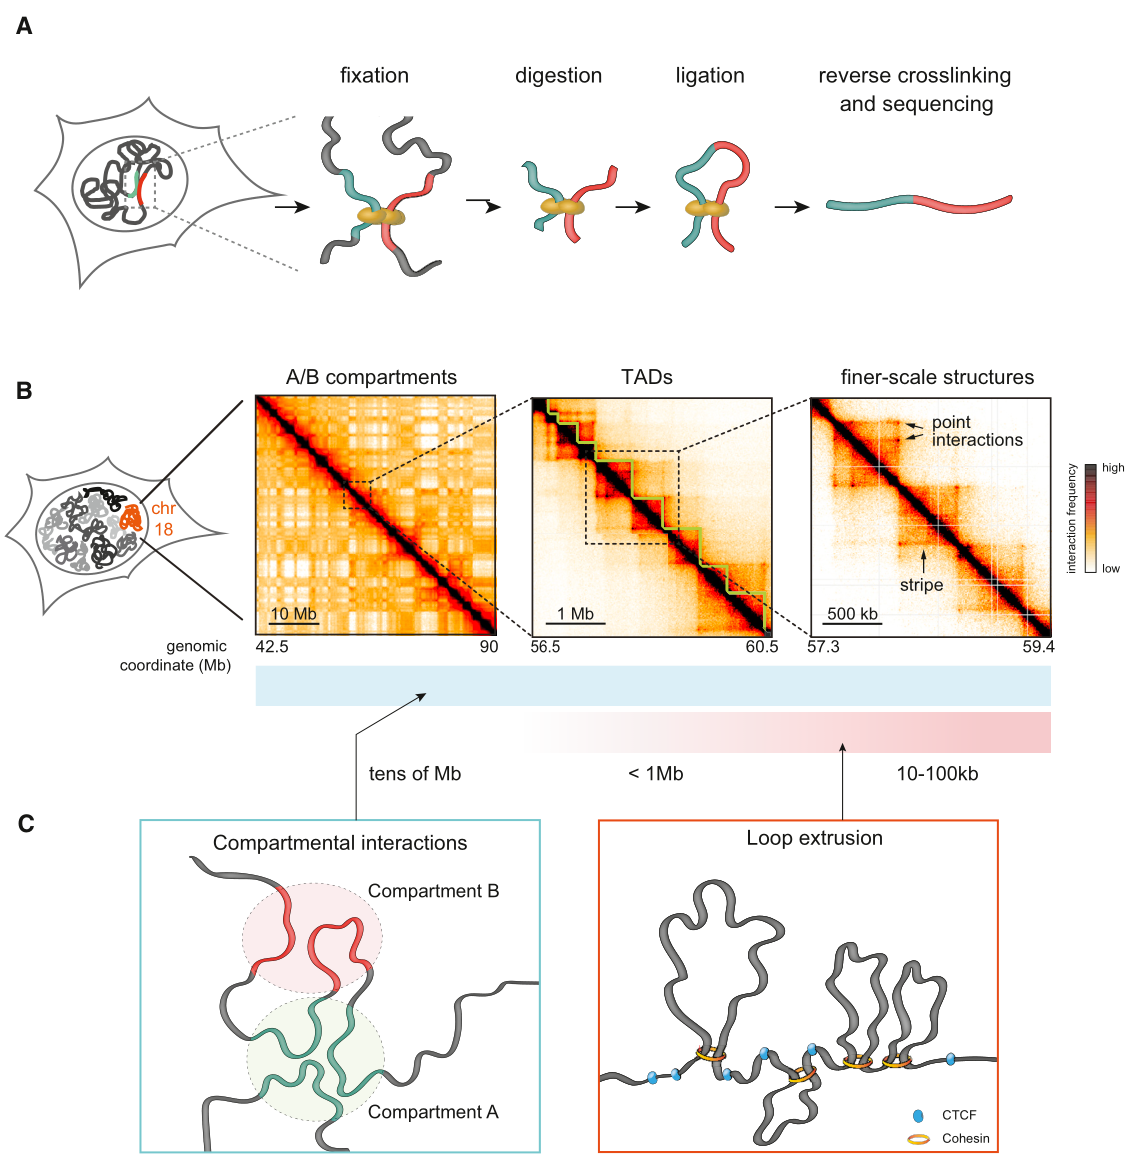
\includegraphics[scale=0.39]{images/fig-2-1.png}
    \end{center}
    \item Limitation of above methods circumvented by a second complementary class of methods, which the authors collectively call \textbf{chromosome conformation capture (3C)}.
        \begin{itemize}
            \item 3C methods use fixation, digestion, and subsequent re-ligation of cross-linked chromatin in order to detect spacial proximity between DNA.
            \item 3C experiments have revealed that each chromosome is folded into complex structural patters emerging at different scales.
                \begin{itemize}
                    \item Active and inactive genomic sequences tend to mutually exclusively associate into A and B compartments, which appear to be formed by attractive interactions of unclear origins.
                    \item Shorter scales (<1 megabase) tend to fold into topologically associating domains (TADs); exact definition ambiguous, but essentially defined as the domains whose boundaries are most conserved during cell differentiation.
                    \item TADs in part mediated by compartmental interactions between active and inactive genes, as well as polycomb-mediated interactions.
                \end{itemize}
            \item The predominant structural features at the TAD level are point-like focal interactions that connect sequences bound by the DNA-binding factor CTCF.
                \begin{itemize}
                    \item CTCF-bound sites occasionally interact across entire domains forming ``stripe''-like structures. Formation of interactions associated with CTCF requires the cohesin complex, which has been proposed to extrude DNA loops until it is arrested by the CTCF bound DNA in a certain orientation or by barrier proteins. 
                \end{itemize}
            \item Together with constraints provided by the nuclear lamina and sub-nuclear compartments, interactions mediated by CTCF-cohesin, compartmental interactions, and poly-comb-coated sequences appear to shape the complex folding of mammalian chromosomes.
        \end{itemize}
    \item Essentially, these discoveries suggest that chromosome structure might play an important role in scaffolding the physical contacts between regulatory sequences, which means they may indirectly affect gene expression during development and homeostasis, as well as participate in other processes such as DNA repair/replication.
        \begin{itemize}
            \item However, some evidence suggest gene expression might not depend on structure, raising various questions:
                \begin{itemize}
                    \item Do chromosomal contacts have direct causal impact on transcription?
                    \item How dynamic are chromosomal interactions?
                    \item How are CTCF/cohesin loops, TAD boundaries, and compartments created?
                    \item Are cooperative interactions between multiple regulatory sequences functionally relevant?
                    \item Are CTCF loops and TAD boundaries causally linked to the accumulation of DNA damage, if so then how?
                    \item Does the 3D structure of chromosomes play a causal role in DNA replication timing?
                    \item How do properties of genome folding relate to the structural properties and shape of the nucleus?
                \end{itemize}
        \end{itemize}
\end{itemize}

\nocite{mccord2020chromosome}
\bibliographystyle{apacite}
\bibliography{summaries.bib}
\end{document}